\chapter{網際內容如何提升教學品質}
\renewcommand{\baselinestretch}{10} %設定行距
%\section{前言}
\par
\renewcommand{\baselinestretch}{2} %設定行距
\fontsize{12pt}\baselineskip\selectfont\qquad 從教學與研究歷程的重要性作為研究動機,希望不只提供學生在學習與研究流程能夠不只留下具體成果,也能有效呈現更細部的歷程資料,以作為學習與研究更有力的佐證資料。
\par

\renewcommand{\baselinestretch}{20} %設定行距
\section{費曼學習法}
\par
\renewcommand{\baselinestretch}{1} %設定行距
\fontsize{12pt}\baselineskip\selectfont\qquad 研究顯示,人類的學習型態分為以下兩種,而當兩種行為同時進行時,能使學習成效大幅提升。
\begin{itemize}
	\item 主動學習
	\item 被動學習
\end{itemize}
\par
\renewcommand{\baselinestretch}{1} %設定行距
\fontsize{12pt}\baselineskip\selectfont\hspace{0.5em} 何謂被動學習? 老師傳播知識,而學生進行吸收,或是透過網路及大眾媒體接收資訊,這些都是常見的被動學習,也是人類大部分獲得知識的渠道。
\par
\renewcommand{\baselinestretch}{1} %設定行距
\fontsize{12pt}\baselineskip\selectfont\hspace{0.5em} 主動學習則是,學習者在接收到資訊後,主動並有意識的思考,在腦中形成一個自己理解方式或產生其他疑問,再去透過尋找資料,主動研究,或是與人討論甚至透過教學等行動進行的學習方式。
\\
\par

\renewcommand{\baselinestretch}{20} %設定行距
\subsection{從費曼學習法的角度觀看}
\par
\renewcommand{\baselinestretch}{1} %設定行距
\fontsize{12pt}\baselineskip\selectfont\qquad 現今華人地區的教學方式,最大的特徵就是「填鴨式」教育。華人的教師認為,他們在課堂上不得不放慢他們習慣的教學進度,因為學生聽不懂也記不住,他們期待學生將聽到的知識記下來,然後就可以應用,可是當這種教育放在國外會發現,很多學生都做不到這一點,他們總是要問「為什麼?,例如:為什麼這條輔助線要劃在這裡,為什麼這道題要這麼算......中方老師的教法,在某種程度上,其實就是一種「填鴨式」,你不需要了解這算法背後的原理,你只需要能夠處理這種算法,學會它並且應用它。可是外國學生對此接受無能,他們沒這個習慣,要在短時間內被「填入」這麼多知識,於是課堂進度被拖慢了。
\par

\renewcommand{\baselinestretch}{20} %設定行距
\subsection{費曼學習法的研究成效}
\par
\renewcommand{\baselinestretch}{1} %設定行距
\fontsize{12pt}\baselineskip\selectfont\qquad 會發現我們的學生會習慣於「接受填鴨」這種僵化的方式去被動學習;反觀外國的學生,在他們的教學體制下,學生會敢於問「為甚麼?」,當他們問出這個問題,並且開始和老師同學討論時,學生就會處於主動學習的狀態了,這時他們的學習效果會大幅提升。\\
\par
\renewcommand{\baselinestretch}{1} %設定行距
\fontsize{12pt}\baselineskip\selectfont\hspace{0.5em} 在生活環境中會有大量的資訊塞入我們的腦中,但是這些資訊屬於被動學習,實際吸收進去的只有不到30\%,而透過研究、紀錄、寫心得甚至教學的方式,與我們腦中的被動資訊相輔相成,可以使資訊吸收的效益增加到80\%~90\%。
\\
\par
\renewcommand{\baselinestretch}{1} %設定行距
\fontsize{12pt}\baselineskip\selectfont\hspace{0.5em} 如(圖\ref{fig.學習金字塔})
\begin{enumerate}
	\item 講課: 授課只是純粹在學生面前說話,不涉及學生的參與,學生只能牢記當中5\% 的知識。
	\item 閱讀: 授課方式增加一個簡報或是參考資料,讓同學邊看邊閱讀,就會稍稍提高到10\%。
	\item 視聽: 授課時播放相關知識的影片,學生的知識牢記率,就會提升到20\%。
	\item 示範: 很多科學科為什麼會特別喜歡做實驗,因為示範比純粹說話好一點,學生的知識牢記率可以提升到30\%。
	\item 小組討論: 當學生直接參與整個學習過程,知識牢記率會大大提升。例如,小組活動,因為這樣就能夠將知識內化成自身的想法,然後再表達出來,這麼知識牢記率就能提升到50\%。
	\item 實踐: 實際動手比看著老師示範好,很多時候科學實驗是老師先做,然後學生再做實際動手,這樣知識牢記率就能提升到80\%。
	\item 教其他人: 最好的知識牢記方法是教其他人,原因是你內化再表達的時候,你會透過不斷教人而增強了對知識的記憶,而達到真正了解、完全吸收資訊。
\end{enumerate}
\par
\renewcommand{\baselinestretch}{1.7} %設定行距
\begin{figure}[hbt!]
\begin{center}
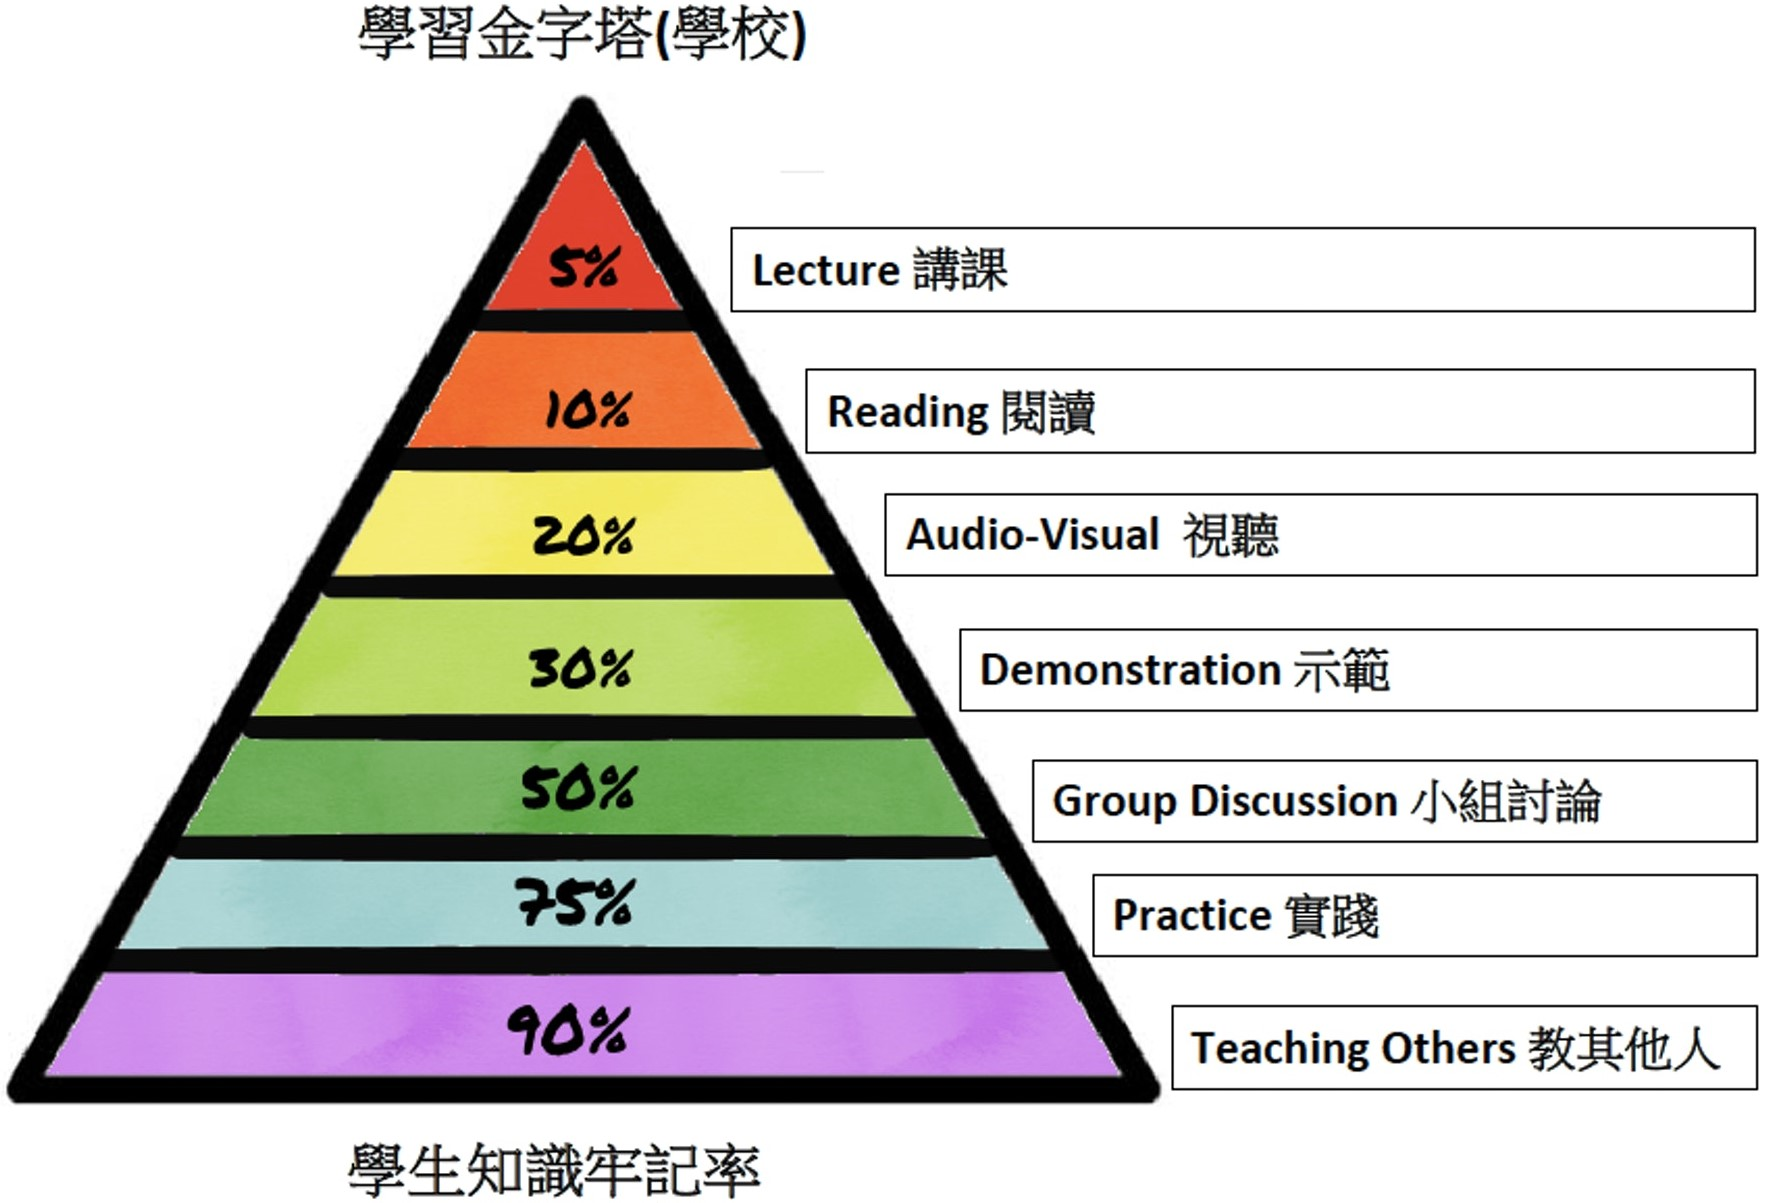
\includegraphics[width=4in]{21}
\caption{\large 學習金字塔}\label{fig.學習金字塔}
\end{center}
\end{figure}
\par

\renewcommand{\baselinestretch}{20} %設定行距
\section{數位化學習環境}
\par
\renewcommand{\baselinestretch}{1} %設定行距
\fontsize{12pt}\baselineskip\selectfont\qquad 於是在數位化的社會下,開始有許多人利用網際內容資源,提供一個數位化學習環境,提升教學品質。\\
\par
\renewcommand{\baselinestretch}{1} %設定行距
\fontsize{12pt}\baselineskip\selectfont\hspace{0.5em} 相比於一般學校裡的教學環境,數位化的網路教學系統可以更容易地設計出讓「使用者主動學習」的教學環境,比如架立討論平台,建立個人專案紀錄歷程檔案......。
\par

\renewcommand{\baselinestretch}{20} %設定行距
\subsection{如何設計出教學環境}
\par
\renewcommand{\baselinestretch}{1} %設定行距
\fontsize{12pt}\baselineskip\selectfont\qquad 首先,我們可以透過費曼學習法,區分主動與被動學習,並分析出教學中,適合引導使用者行主動學習的要素,如以下的方式。
\begin{enumerate}
	\item 課程目標
	\begin{itemize}
		\item 為什麼要開這門課?
		\item 開這門課的目的是什麼?
		\item 希望達成什麼樣的目標?
		\item 希望解決什麼樣的問題?
		\item 達成這樣的目標對於個人、社會、世界會發生什麼樣的影響?
	\end{itemize}
	\item 理論基礎
	\begin{itemize}
		\item 為達成前述的目標,應該要如何結構一門課?
		\item 什麼樣的理論基礎及知識觀點可以支撐起這個架構?
	\end{itemize}
	\item 教學題材
	\begin{itemize}
		\item 選用什麼題材可以反應真實世界概況?
		\item 什麼實例可以串接學生及生活世界之間的距離?
		\item 什麼內容可以與時俱進並體現時代的脈動?
	\end{itemize}
「教學」中值得「研究」的元素
	\item 教學方法
	\begin{itemize}
		\item 設計何種教法可以合適地表達教材的意義?
		\item 規劃什麼樣的活動可以激發學生的動機,並且深化學習的意義?
	\end{itemize}
	\item 學生學習
	\begin{itemize}
		\item 學生如何建構對於知識的理解?
		\item 如何形成相關的態度?
		\item 學生學習及認知的過程為何?
	\end{itemize}
	\item 成果評量
	\begin{itemize}
		\item 經過教學之後,整體課程的效果如何?
		\item 如何明確地評量?
	\end{itemize}
\end{enumerate}
\par

\renewcommand{\baselinestretch}{20} %設定行距
\section{數位教育資源的實體功能}
\par
\renewcommand{\baselinestretch}{1} %設定行距
\fontsize{12pt}\baselineskip\selectfont\qquad 分析完教學中,適合引導使用者主動學習的要素後,針對上述要點,我們可以規劃出一系列的教學網站結構。
\begin{enumerate}
	\item 測驗練習: 用軟體做題,不用等待老師長時間的批改,自己馬上就能知道自己的薄弱環節。
	\item 測驗詳解: 測驗完,針對自己不太會的,可以看到答題詳解,立即更正原本錯誤的觀念。
	\item 互動平台: 傳統的課堂,由於時間有限,無法廣泛聽取所有同學的觀點,再加上青春期的特點,即使有想法,有些孩子也總是羞於舉手回答,一定程度上影響了表達和共享,老師也很難知道學生的情況。課堂交流也不一定要面對面,讓學習跨越時空,一對一的課堂問答模式變成了面向全體的在線問答。多對多課堂模式,所有學生都可以看到「班級問答」區的問題,如此,交流不再是少部分同學的特權,每個人的機會都是均等的,這也在某種程度上重塑學生學習的信心。在線問答和交流,所有孩子都有機會及時整理自己的知識和想法,老師也能真正和孩子們互動起來。這種模式下的學習,打破了課堂時間和空間位置的束縛,增大信息流量,實現全班同學的思維互動。同時,也發揮了部分學有餘力的同學的資源優勢,最終提高了全體學生的學習積極性和學習績效。
	\item 個人紀錄: 查看已發觀點並進行適當地調整,最終將自己的觀點整理輸出。
	\item 背景後台: 針對不同的使用者,開放不同的權限,老師可以上傳了海量的學習資源,一鍵將不同難度的視頻推送給不同層次的學生;利用它進行課堂學習,同時也能給程度不一致的學生設置不同的課後習題,並且觀察到後台大數據,瞬間分析出每一個學生的作業正確率和做題速度等,每個學生解題答案老師一清二楚。
\end{enumerate}
\par
\renewcommand{\baselinestretch}{1} %設定行距
\fontsize{12pt}\baselineskip\selectfont\hspace{0.5em} 將教師從知識的搬運工變成課堂教學活動的設計者、組織者、指導者與參與者;把學生從知識的背誦者、接受者變為知識的實踐者、探索者和創造者,自動學習,學會分享交流,並在討論中觸發創新,實現自主化、個性化的學習。
\par

\renewcommand{\baselinestretch}{20} %設定行距
\section{網際網路-遠距新趨勢}
\par
\renewcommand{\baselinestretch}{1} %設定行距
\fontsize{12pt}\baselineskip\selectfont
\begin{enumerate}
	\item 電子郵件: 學生可利用電子郵件接收課程教材、作業分配、班級的相關資訊、並與教師、同學或不同年紀的學生相互溝通。教師也可另外設定一個課程討論群組(course listserv),所有的討論和問題都會寄到課程討論群組的電子郵件寄住信箱來,系統會自動將這些内容再寄給各組成員。
	\item 公告欄: 學生直接將自己的討論和間題張貼(post)在公告欄、公開討論區或新閒群組上,以相互溝通。使用者必須連到主機伺服器去閱覽這些文章。這樣可以有組纖的交談,因爲使用者可以選擇自己有興趣的主題進行閱讀和回應。
	\item 資料下載
學生可透過以下幾種方式獲取教學資料:利用檔案傳輸下載文件、教材或軟體;公告欄下載主題文章:全球資訊網下載所需的資料。這些資料下載之後:可在學生的電腦中閱讀或列印。這種方式最缺乏互動性,但卻是透過網際網路進行遠距教學或训練最常使用的方式。
	\item 互動式個別指導教材(Interaotive tutorial)
學生連線到網際網路上(通常是全球資訊網,並在線上取得個別指導教材。道些教材包括閱讀資料、連結到新的網站、回答問題或測驗等。有些個別指導教材允許學生依照自己的速度進行學習,每次連線進來都可繼續上次未完成的學習。
	\item 即時互動會議系統(Real-time Conference)
電子佈告欄和電子郵件在遠距學習的環境中屬於非同步學習。而「即時互動會議系統」則屬於同步學習,教師與學生同時在線上進行面對面的教學與討論。這是最接近傅統教室教學情境的一種方式,教師與學生或學生之間可即時的交談與間答。即時互動會議系統可採用多物件導向系統(Muti-user Object Oriented; MOOs),這是一個可以讓許多使用者同時進入的互動系統,例如網路聊天室 (Internet Relay Chat ; IRC) 便提供了許多即時學習和互動的機會。
	\item 全球資訊網: 以多媒體的方式(如文字、圖片。影像、動畫、聲音,等)提供各式各樣的資訊。大部份全球賌訊網的瀏覽器可以同時使用檔案找尋系統(Archie)、檔案傳輸、資料查詢服務系統、新閒論壇、電子郵件等資源。教師與學生可利用上述資源搜尋、列印、和下載資訊。全球資訊網不僅能夠整合網路的資源,還可讓使用者以建立網頁(Homepage)的方式,來成爲個人資訊提供者,而不單只是一個資訊使用者。道種整合運用資訊及讓使用者參與資訊建設的功能,使全球資訊網成為不可忽融的新教學媒體。
\end{enumerate}
\par












